%------------------------------------------%
% Cannabis Data Science
% Date: 2/9/2022
%------------------------------------------%
\documentclass[xcolor={dvipsnames}]{beamer}
\hypersetup{pdfpagemode = FullScreen}
\mode<presentation>{
  \usetheme{Boadilla}
  \usecolortheme{orchid}
  \usefonttheme{default}
  \setbeamertemplate{navigation symbols}{}
  \setbeamertemplate{caption}[numbered]
}
\setbeamersize{
  text margin left = 0.5in,
  text margin right = 0.5in
}

%------------------------------------------%
% Title
%------------------------------------------%
\title[\textbf{Cananbis Data Science \#52}]{}
\author{Cannabis Data Science}
\institute[]{\Large Cananbis Data Science \#52}
\date{February \nth{9}, 2022}

%------------------------------------------%
% Packages
%------------------------------------------%
\usepackage[english]{babel}
\usepackage[utf8x]{inputenc}
\usepackage{tikz} % For styling.
\usepackage{xparse}

%------------------------------------------%
% Colors
%------------------------------------------%
%\usepackage[dvipsnames]{xcolor}
\definecolor{Green}{RGB}{34, 153, 84}
\definecolor{LightGreen}{RGB}{218, 247, 166}
\definecolor{DarkGreen}{RGB}{2, 48, 32}
\definecolor{Orange}{RGB}{255, 87, 51}
\definecolor{DarkOrange}{RGB}{199, 0, 57}
\definecolor{Yellow}{RGB}{255, 195, 0}

%------------------------------------------%
% Theme
%------------------------------------------%
\setbeamercolor*{palette primary}{bg=LightGreen, fg=DarkGreen}
\setbeamercolor*{palette secondary}{bg=LightGreen, fg=DarkGreen}
\setbeamercolor*{palette tertiary}{bg=LightGreen, fg=DarkGreen}
%\setbeamercolor*{palette quaternary}{bg=myNewColorD, fg = green}

%------------------------------------------%
% Packages
%------------------------------------------%
\usepackage{amsmath}
\renewcommand*\footnoterule{} % No separating line on footnote.
\usepackage{mathtools} % For annotating equations.
\usepackage{hhline} % for double bars.
\usepackage[super]{nth} % For formatting 1st, 2nd, 3rd, etc.
\usepackage{graphicx, caption, subcaption}

%------------------------------------------%
% Commands
%------------------------------------------%

% Top space.
\newcommand\T{\rule{0pt}{2.5ex}}

% Bottom space.
\newcommand\B{\rule[-1.25ex]{0pt}{0pt}}

% Blocks.
\newenvironment<>{Block}[2][.9\textwidth]
  {\setlength{\textwidth}{#1}
  \begin{actionenv}#3
    \def\insertblocktitle{#2}\par
    \usebeamertemplate{block begin}}
  {\par\usebeamertemplate{block end}
  \end{actionenv}}

% Balls.
\defbeamertemplate{enumerate item}{largeball}
{\begin{pgfpicture}{-1ex}{-0.65ex}{1.5ex}{1.5ex}
\usebeamercolor[fg]{item projected}
{\pgftransformscale{2.5}\pgftext{\Large\pgfuseshading{bigsphere}}}
{\pgftransformshift{\pgfpoint{0pt}{0.5pt}}
\pgftext{\usebeamerfont*{item projected}\small\insertenumlabel}}
\end{pgfpicture}}

% Fancy arrows.
\NewDocumentCommand\UpArrow{O{2.0ex} O{black}}{%
   \mathrel{\tikz[baseline] \draw [->, line width=0.5pt, #2] (0,0) -- ++(0,#1);}} % Fancy up-arrow.
\NewDocumentCommand\DownArrow{O{2.0ex} O{black}}{%
   \mathrel{\tikz[baseline] \draw [<-, line width=0.5pt, #2] (0,0) -- ++(0,#1);}} % Fancy down-arrow.

% Equations with numbers on the left.
\makeatletter
\newcommand{\LeftEqNo}{\let\veqno\@@leqno}
\makeatother

%------------------------------------------%
% Presentation
%------------------------------------------%
\begin{document}

% Title page.
\begin{frame}{}
  
\includegraphics[scale=0.33]{images/logo.pdf}
  \vspace*{-2\baselineskip}
  \titlepage
\end{frame}

%------------------------------------------%
% Introduction
%------------------------------------------%
\section{Introduction}

\begin{frame}{}

\begin{center}
\begin{minipage}{.9\linewidth}
\begin{Block}{Question of the Day}

\vspace{\baselineskip}

How does cannabis move through the industry?

\vspace{\baselineskip}

\end{Block}
\end{minipage}
\end{center}

\begin{figure}
\begin{subfigure}[t]{.9\textwidth}
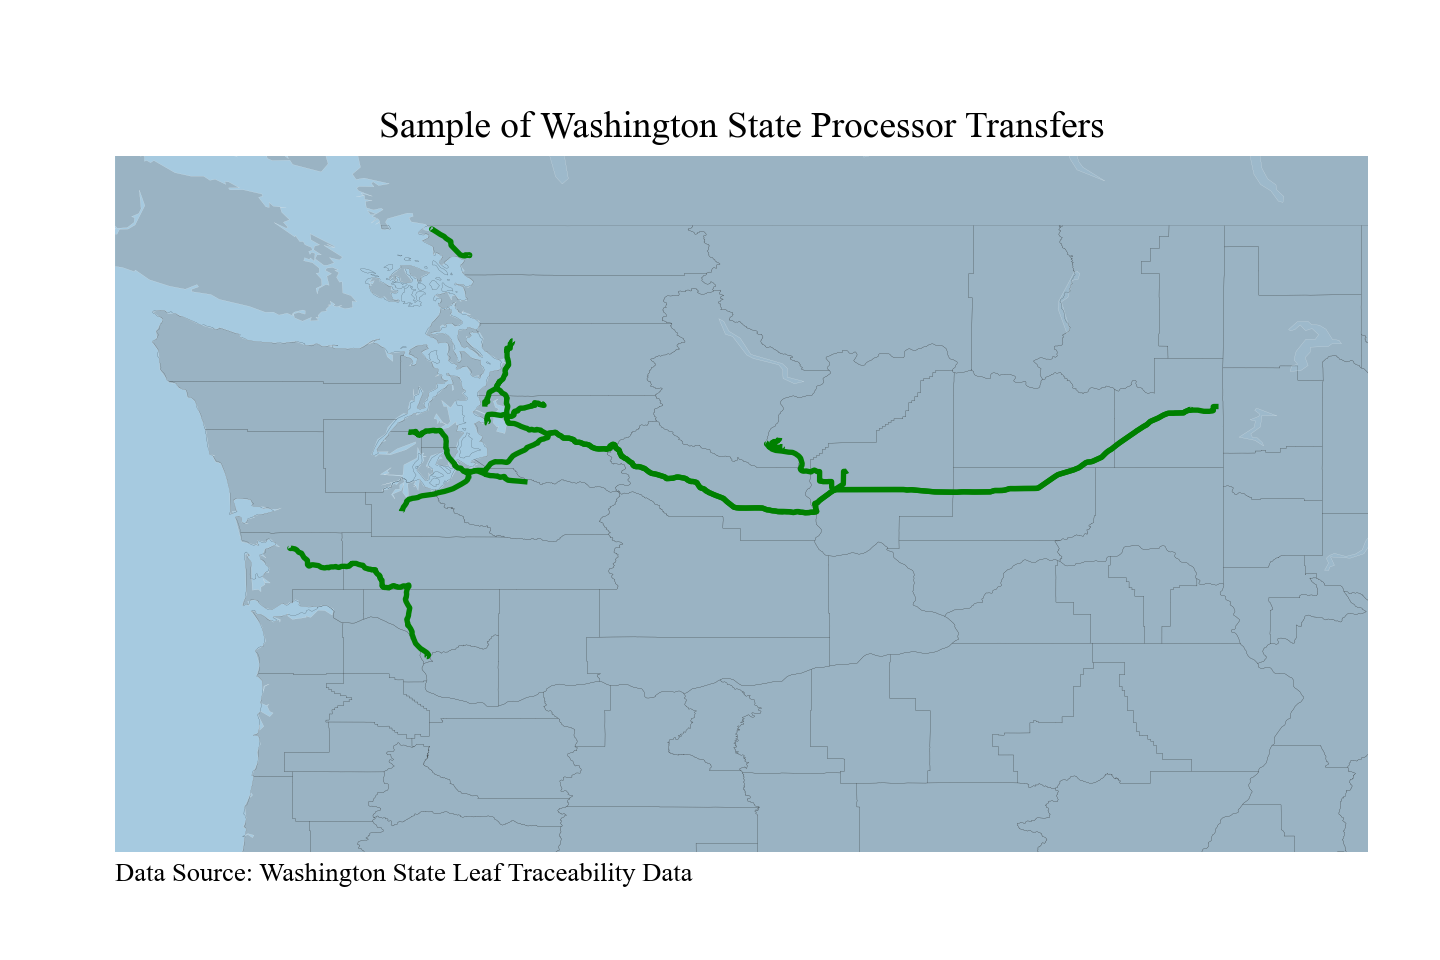
\includegraphics[width=\textwidth]{images/transfers-map-processors.png}
\end{subfigure}
\end{figure}

\end{frame}


%------------------------------------------%
% Panel Data
%------------------------------------------%
\section{Panel Data}

\begin{frame}{}

{\large \textbf{Panel Data}}\vspace{1.5\baselineskip}\\

\begin{itemize}

\item A panel has the form
\vspace{.5\baselineskip}

\begin{figure}
    \begin{subfigure}[t]{.5\textwidth}
      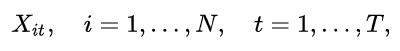
\includegraphics[width=\textwidth]{images/panel.png}
    \end{subfigure}
\end{figure}

where
\vspace{.5\baselineskip}
\begin{itemize}
\item $i$ is the individual dimension and
\item $t$ is the time dimension.
\end{itemize}
\vspace{1.5\baselineskip}

\item We can look at {\bfseries total transfers} ($x_{it}$) by \newline licensee or license type ($i$) \newline over time ($t$).

\end{itemize}


%A general panel data regression model is written as
%
%\begin{figure}
%    \begin{subfigure}[t]{.3\textwidth}
%      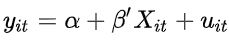
\includegraphics[width=\textwidth]{images/regression.png}
%    \end{subfigure}
%\end{figure}
%
%where
%
%\begin{figure}
%    \begin{subfigure}[t]{.25\textwidth}
%      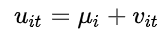
\includegraphics[width=\textwidth]{images/errors.png}
%    \end{subfigure}
%\end{figure}
%
%Estimation with a \textbf{fixed effects} or \textbf{random effects} model depends on assumptions about $\mu_i$, the individual-specific, time-invariant effects.

\end{frame}


%------------------------------------------%
% Data science history.
% % TODO: Add text + visualizations
%------------------------------------------%
%\section{Data Science History}
%\begin{frame}{}
%
%{\large \textbf{A Brief History Lesson on Data Science}}\vspace{0.5\baselineskip}\\
%
%%Bayes and Bayes Theorem
%%
%%The idea is that Bayes Theorem encapsulates how people, including researchers, make decisions. So, it is of utmost importance to state all of your prior beliefs, quantify your beliefs as much as possible, then update your beliefs when exposed to new data, given its characteristics and probability of occurring.
%%
%%When you use Bayesian methodology you acknowledge your fallibility and that you come to every choice you make with preexisting data and beliefs.
%
%\end{frame}

%------------------------------------------%
% Cannabis cultivation history.
% % TODO: Add text + visualizations
%------------------------------------------%
%\section{Cannabis Cultivation History}
%\begin{frame}{}
%
%{\large \textbf{A Brief History Lesson on Cannabis Cultivation}}\vspace{0.5\baselineskip}\\
%
%
%\end{frame}

%------------------------------------------%
% Statistics of Big Data
%------------------------------------------%
%\section{Statistics of Big Data}
%\begin{frame}{}
%
%{\large \textbf{Statistics of Big Data}\vspace{1.5\baselineskip}\\
%\begin{itemize}
%
%% TODO: Talk about big data and statistics...
%
%\end{frame}

%------------------------------------------%
% Augmenting and visualizing data.
% TODO: Add visualizations
%------------------------------------------%
%\section{Augmenting and Visualizing Data}
%\begin{frame}{}
%
%{\large \textbf{Augmenting and visualizing cannabis data}}\vspace{1.5\baselineskip}\\
%\begin{itemize}
%
%\item {\bfseries Box (and Swarm) Plots} - Useful for visualizing variability.
%
%\vspace{\baselineskip}
%
%\item {\bfseries Bubble Plots} - Useful for visualizing a third dimension in a 2D plot.
%
%\vspace{\baselineskip}
%
%\item {\bfseries Scatter Plots} - Useful for visualizing the space dimension of your data.
%
%\end{itemize}
%
%\end{frame}


%It is imperative to have the right tools for the task at hand.
%
%The idea is to merge objects by a common factor and retain the data points, or fields, that you need in your analysis. Once you have merged two or more datasets, keeping all or some of the fields and data points, then you have created an augmented dataset, creating value by facilitating analyses that are only possible with the combination of data.
%
%There is a fixed cost of augmenting data; the know--how, the equipment, the time and energy required to process the data, however, once created the augmented data can be supplied at extraordinarily low costs. It would be efficient, in the long run, to supply data at (almost) the rate that it is demanded. The price would approach the average fixed cost, which would approach 0 as the number of datasets demanded increases. Thus, it appears at first glance that data markets are remarkably efficient markets and provide great benefit to both data suppliers and consumers.
%
%The analyses that can be performed on augmented datasets are bountiful. Just to name a few, you can augment data with geographic, time, individual, and group--level data.
%
%Geographic data lends itself to beautiful visualizations.



%------------------------------------------%
% DONE: About Processing
%------------------------------------------%

%% Figures
%\begin{figure}
%    \begin{subfigure}[t]{.425\textwidth}
%      \begin{center}
%      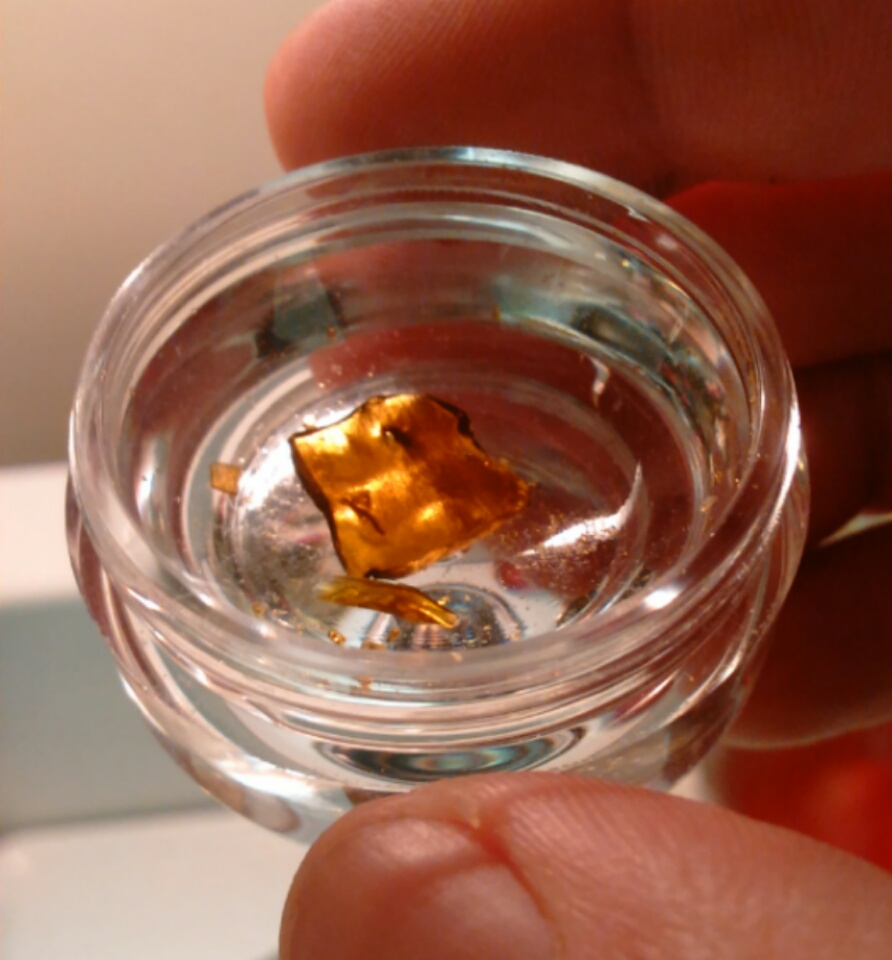
\includegraphics[height=4cm]{images/shatter.jpg}
%      \end{center}
%      \caption*{A cannabis concentrate, known as shatter, produced in Alaska (74\% THC)\vspace{0.5\baselineskip}\\ \tiny Author: Cameek33 at English Wikipedia\newline CC BY-SA 4.0\newline https://creativecommons.org/licenses/by-sa/4.0/\newline No changes were made to the image.}
%    \end{subfigure}%
%    \hspace{.075\textwidth}
%    \begin{subfigure}[t]{.425\textwidth}
%      \begin{center}
%      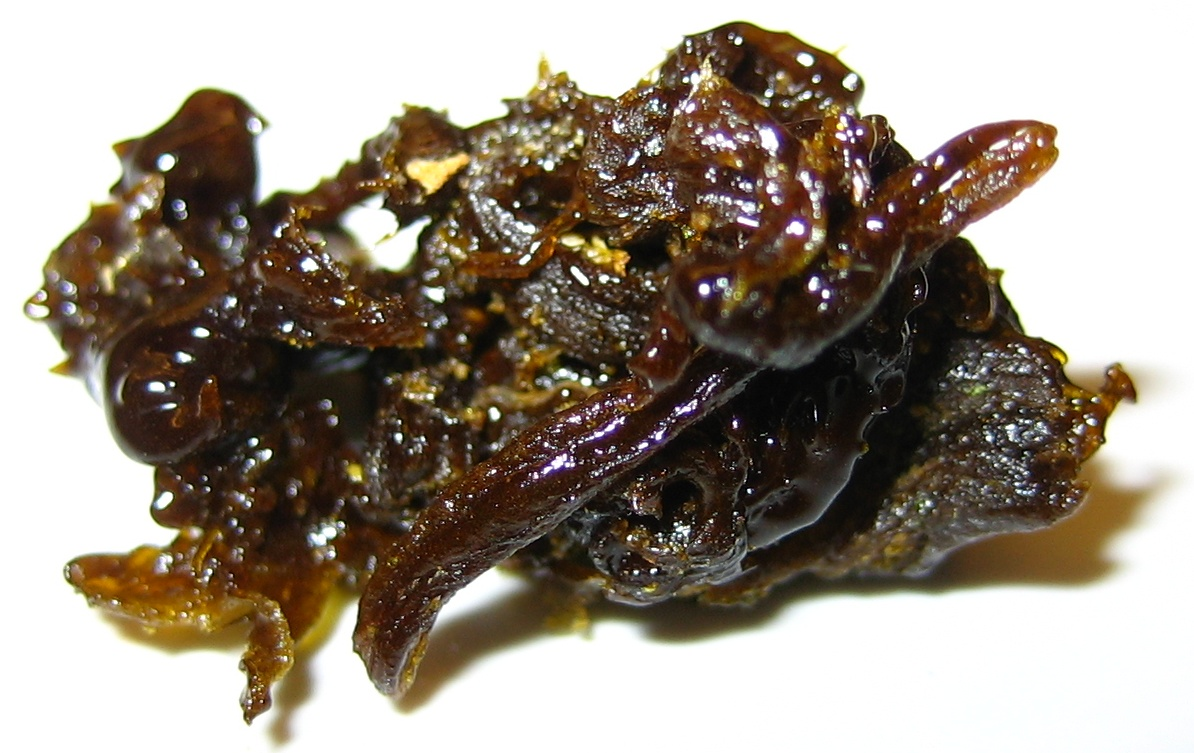
\includegraphics[height=4cm]{images/hemp-oil.jpg}
%      \end{center}
%%      \caption*{Hemp extract (``hash oil'').}\vspace{0.5\baselineskip} \tiny Auhtor: Erik Fenderson (2006)\newline Public Domain.}
%    \end{subfigure}
%\end{figure}

%------------------------------------------%
% DONE: History of processing
%------------------------------------------%

%\begin{frame}{}
%
%{\large \textbf{History of Cannabis Processing}}\vspace{0.5\baselineskip}\\
%
%Humans are remarkably good at using plants as factories of complex chemicals.
%
%\begin{itemize}
%
%\item Cannabis may have been used in India as early as 1000 BC.
%
%\end{itemize}
%
%\begin{figure}
%  \begin{center}
%    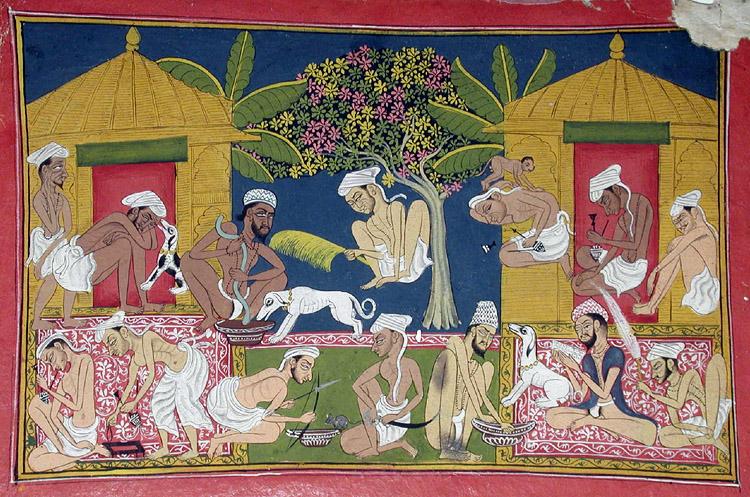
\includegraphics[height=4cm]{images/bhang-eaters.jpg}
%   \end{center}
%   \caption*{hang eaters from India c. 1790.\vspace{0.5\baselineskip}\\ \tiny This work is in the public domain in its country of origin and other countries and areas where the copyright term is the author's life plus 100 years or fewer.}
%\end{figure}
%
%\end{frame}

%------------------------------------------%
% DONE: Cannabis Edibles
%------------------------------------------%

%\begin{frame}{}
%
%{\large \textbf{Cannabis Edibles}}\vspace{0.5\baselineskip}\\
%
%\begin{itemize}
%
%\item {\itshape\small ``The first cannabis edible recipe appeared in the United States in the early 1960s in a cookbook called The Alice B. Toklas Cookbook written by Alice B. Toklas. The recipe is called ``Hashish Fudge'' and was actually contributed by Alice's good friend, Brion Gysin''}
%
%\item {\itshape\small ``The 1001 Nights provided him ``with an entr\{'}ee into Tangiers society. His Moroccan culinary delights even merited an entry in Alice B. Toklas's famous cookbook, with a recipe for hashish fudge. Toklas, however, had no idea what the mysterious ingredient – cannabis.''
%
%\item {\itshape\small ``A mixture of fruit, nuts, spices, and ``canibus sativa''.''}
%
%\end{itemize}
%
%% Figures
%\begin{figure}
%    \begin{subfigure}[t]{.425\textwidth}
%      \begin{center}
%      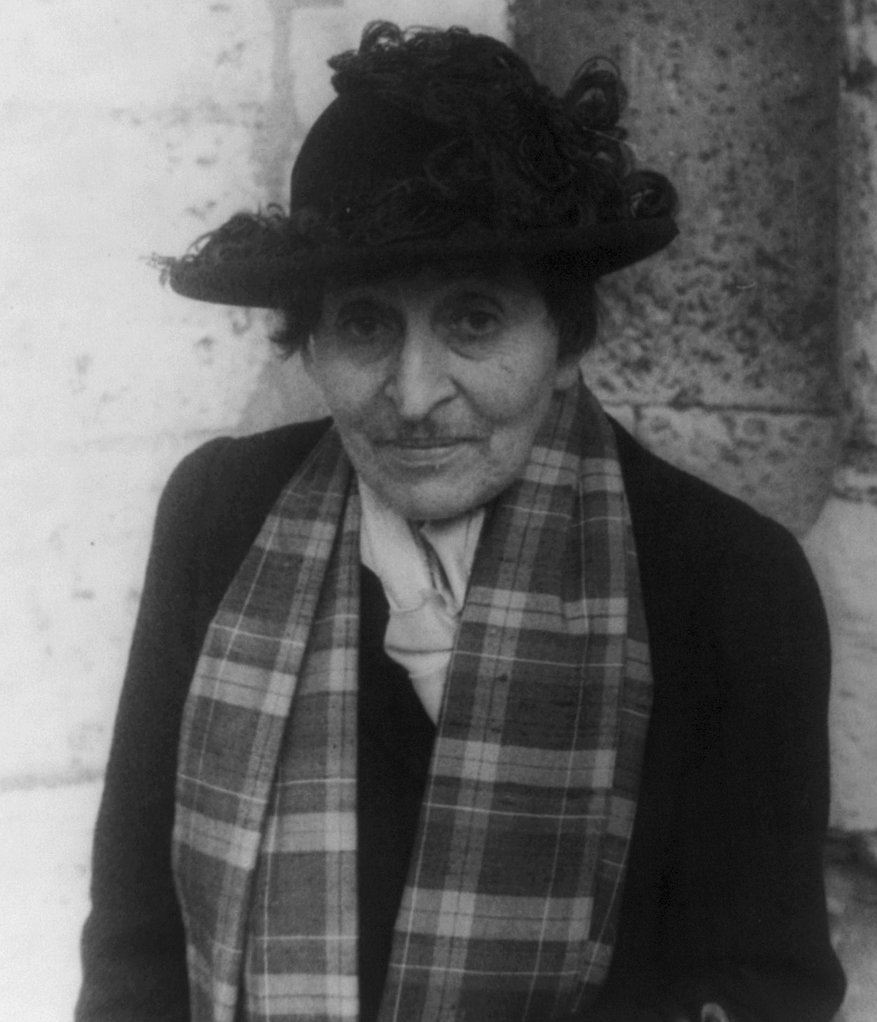
\includegraphics[height=4cm]{images/alice-b-toklas.jpg}
%      \end{center}
%      \caption*{Alice B. Toklas (1877 – 1967).\vspace{0.5\baselineskip}\\ \tiny Author: Carl Van Vechten (1949)\newline Public Domain\newline No changes were made to the image.}
%    \end{subfigure}%
%    \hspace{.075\textwidth}
%    \begin{subfigure}[t]{.425\textwidth}
%      \begin{center}
%      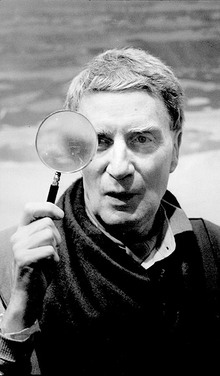
\includegraphics[height=4cm]{images/Brion-Gysin.jpg}
%      \end{center}
%      \caption*{John Clifford Brian Gysin (916 - 1986).\vspace{0.5\baselineskip} \tiny\newline Public Domain.}
%    \end{subfigure}
%\end{figure}
%
%\end{frame}

%------------------------------------------%
% REDO? Separations
%------------------------------------------%

%\begin{frame}{}
%
%{\large \textbf{Cannabinoid Separations}}\vspace{0.5\baselineskip}\\
%
%\begin{itemize}
%
%\item First cannabinoid, CBN, fully formed by Robert S. Cahn (chemist) in 1940.
%
%\item CBD discovered by Roger Adams (chemist) in 1942.
%
%\item First stereochemistry of CBD (cannabidiol) by Raphael Mechoulam (professor) in 1963.
%
%\item First stereochemistry of THC (tetrahydrocannabinol) by Raphael Mechoulam in 1964.
%
%\end{itemize}
%
%%\begin{figure}
%%  \begin{center}
%%    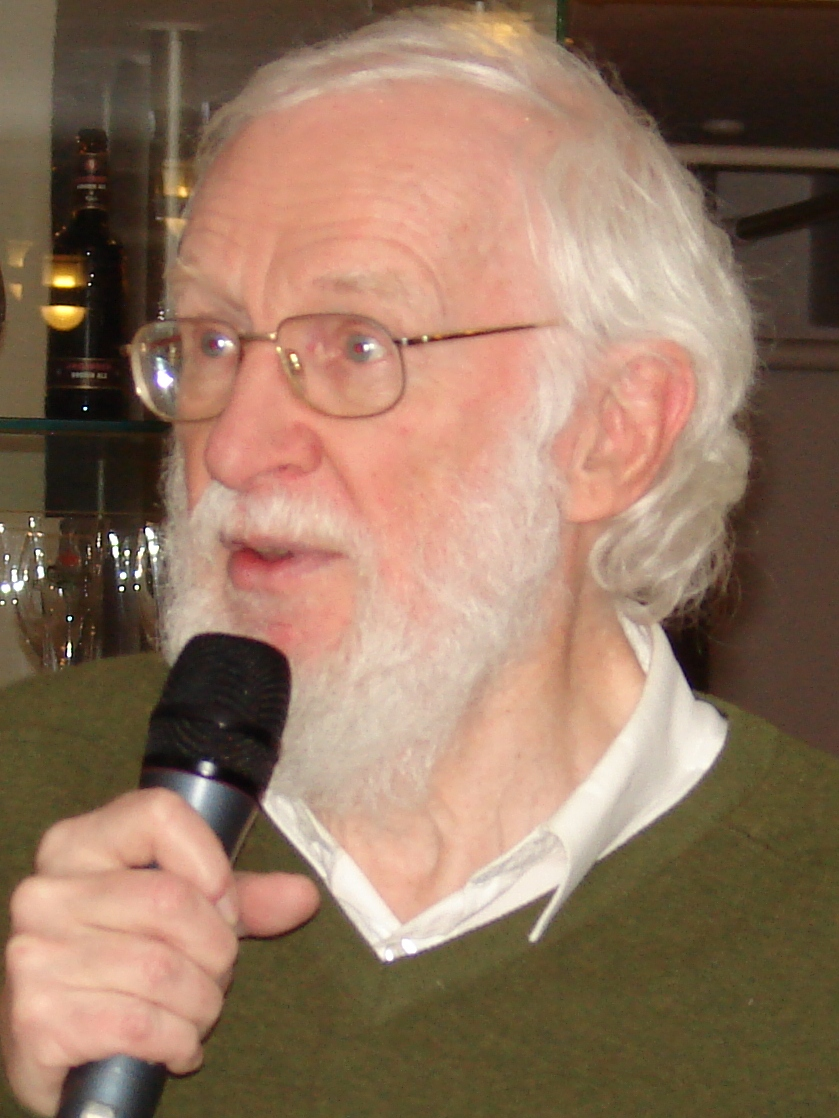
\includegraphics[height=4cm]{images/Peternaur.jpg}
%%   \end{center}
%%   \caption*{hang eaters from India c. 1790.\vspace{0.5\baselineskip}\\ \tiny Author: Tzachi Lerner \newline The copyright holder of this file allows anyone to use it for any purpose, provided that the copyright holder is properly attributed. Redistribution, derivative work, commercial use, and all other use is permitted.}
%%\end{figure}
%
%\end{frame}

%------------------------------------------%
% TODO: Chemistry of processing
%------------------------------------------%

%\begin{frame}{}
%
%{\large \textbf{Chemistry of Cannabis Processing}}\vspace{0.5\baselineskip}\\
%
%\begin{itemize}
%
%\item Many cannabinoids are orally bioactive after chemical conversion, in particular from temperature.
%
%\item The decarboxylation reaction of THCA to THC occurs at 230 \degree F (110 \degree C).
%
%\item The boiling point of THC is 315 \degree F (157 \degree C)
%
%\item Other notable boiling points:
%
%%\begin{itemize}
%%
%%\item CBD	320 \degree F (160 \degree C) - 356 \degree F (180 \degree C).
%%
%%\item Delta-8-THC	347 \degree F (175 \degree C) - 352 \degree F (178  \degree C).
%%
%%\item THCV at < 220 \degree F (104.5 degree C).
%%
%%\end{itemize}
%
%\end{itemize}
%
%{\tiny Reference: McPartland & Russo, 2001}
%
%\end{frame}

%------------------------------------------%
% DONE: Cannabinoid Separation
%------------------------------------------%

%\begin{frame}{}
%
%{\large \textbf{Cannabinoid Separation}}\vspace{0.5\baselineskip}\\
%
%{\itshape ``Cannabinoids can be separated from the plant by extraction with organic solvents. Hydrocarbons and alcohols are often used as solvents. However, these solvents are flammable and many are toxic. Butane may be used, which evaporates extremely quickly. Supercritical solvent extraction with carbon dioxide is an alternative technique. Once extracted, isolated components can be separated using wiped film vacuum distillation or other distillation techniques.[59] Also, techniques such as SPE or SPME are found useful in the extraction of these compounds.''}
%
%\end{frame}


%------------------------------------------%
% TODO: Processing Edibles
%------------------------------------------%

%\begin{frame}{}
%
%{\large \textbf{Processing Cannabis Edibles}}\vspace{0.5\baselineskip}\\
%
%% "Ingesting cannabis may produce effects that last longer and can be more intense than inhaling cannabis"
%
%% "The important base to all food edibles is that it has fat that has been infused with THC.[28] In other words, any food that contains butter, oil, milk, or any fatty substance can be turned into an edible."
%
%% Figure
%% THC-infused gummies (5mg of THC each).
%% Author: Elsa Olofsson at cbdoracle.com (2020)
%% License: CC BY 2.0 https://creativecommons.org/licenses/by/2.0/deed.en
%% No changes were made to the image.
%
%\end{frame}


%\begin{frame}{}
%
%{\large \textbf{Cannabis Products}}\vspace{0.5\baselineskip}\\
%
%% Tinctures
%
%% "Tinctures are potent, alcohol-based cannabis extracts.[29] The solubility of THC in ethanol is greater than 1 g/mL.[32] They are considered edibles as they are meant to be absorbed through the mouth and tongue."
%
%\end{frame}


%------------------------------------------%
% DONE: About variability.
%------------------------------------------%

%\begin{frame}{}
%
%{\large \textbf{Cannabis Processing Variability}}\vspace{0.5\baselineskip}\\
%
%Reasons processors may be concerned about variability:
%
%\begin{itemize}
%
%\item For financial reasons: Minimize risk.
%
%\item For economic reasons: People are risk adverse.
%
%\item For engineering reasons: Minimize variance.
%
%\item For business, marketing, and public health reasons: Maximize consistency.
%
%\end{itemize}
%
%\end{frame}


%------------------------------------------%
% Takeaway
%------------------------------------------%
\section{Takeaway}
\begin{frame}{}

\begin{center}
\begin{minipage}{3.85in}

% Thank you.

\includegraphics[width=.25in]{images/prayer.png} {\Large \textbf{Thank you for coming.}}\\

% Re-cap the lesson of the week.
\begin{center}
\begin{minipage}{.9\linewidth}
\begin{Block}{Lessons of the Day}

\vspace{\baselineskip}

\begin{itemize}

\item Observing how cannabis moves through the economy can lend unique insights.

\vspace{\baselineskip}

\end{itemize}

\end{Block}
\end{minipage}
\end{center}

\vfill

\end{minipage}
\end{center}

\end{frame}


%------------------------------------------%
% End
%------------------------------------------%
\end{document}
